% =====================================================================
%  Trajectory Optimisation for a Steerable Airdrop in Unknown Wind
%  Project synopsis -- IMRaD
%
%  Compile: pdflatex synopsis  (twice, for cross-references)
%
%  Figures required in ./figures/ :
%     drop_none.png            Fig 1(a)  screenshot from docs/ (no estimate)
%     drop_ekf.png             Fig 1(b)  screenshot from docs/ (EKF)
%     fig1a_no_estimate.png    Fig 2(a)
%     fig1b_ekf_estimate.png   Fig 2(b)
%     design_chart.png         Fig 3
%  All are generated title-less; captions carry the text.
%
%  Fig 1 is captured from the interactive page at
%    wind 2.0 m/s, direction 90 deg, height 30 m, loading 1.20, bias +10 deg
%  Retaking it is just a matter of overwriting those two files.
% =====================================================================

\documentclass[11pt,a4paper]{article}

\usepackage[margin=2.4cm]{geometry}
\usepackage{graphicx}
\usepackage{amsmath}
\usepackage{booktabs}
\usepackage{caption}
\usepackage{subcaption}
\usepackage{xcolor}
\usepackage{fancyhdr}
\PassOptionsToPackage{hyphens}{url}
\usepackage[hidelinks]{hyperref}
\usepackage{cleveref}
\Urlmuskip=0mu plus 1mu\relax
\usepackage{times}

\captionsetup{font=small,labelfont=bf,skip=6pt}
\captionsetup[sub]{font=small,justification=raggedright,singlelinecheck=false}
\setlength{\parskip}{4pt}
\setlength{\parindent}{0pt}

% ------------------------------------------------- header / footer (minimal)
\definecolor{accent}{HTML}{3A5BA0}

% Change this one word if the class is different.
\newcommand{\theclass}{Class XII}

\pagestyle{fancy}
\fancyhf{}
\fancyhead[C]{\footnotesize\textsc{Trajectory Optimisation for a Steerable Airdrop in Unknown Wind}}
\fancyfoot[L]{\footnotesize\textsc{\theclass\ $\cdot$ Atomic Energy Central
School, Mysuru}}
\fancyfoot[R]{\footnotesize\thepage}
\renewcommand{\headrule}{\color{accent}\hrule height 0.4pt}
\renewcommand{\footrulewidth}{0pt}
\setlength{\headheight}{14pt}


\begin{document}

% ---------------------------------------------------------------- COVER PAGE
\begin{titlepage}
\thispagestyle{empty}
\centering

\vspace*{3.2cm}

{\LARGE\bfseries TRAJECTORY OPTIMISATION FOR A\\[8pt]
STEERABLE AIRDROP IN UNKNOWN WIND\par}

\vspace{14pt}
{\large Guiding Packages to a Target for Relief Distribution,\\[4pt]
with No Wind Sensor on Board\par}

\vspace{26pt}
{\textsc{Atomic Energy Central School, Mysuru}\par}

\vfill

\includegraphics[width=4.4cm]{logo.png}
\vfill

{\large BY: AMULYA D\par}

\vspace{6pt}
{\footnotesize Interactive version:
\url{https://1101-hub.github.io/guided-airdrop/}\par}

\vspace{10pt}
{\color{accent}\rule{\textwidth}{0.8pt}}

\vspace*{0.6cm}
\end{titlepage}

% ---------------------------------------------------------------- ABSTRACT
\section*{Abstract}

Relief supplies airdropped to flood-isolated communities drift with the wind and
land away from the intended point. This work simulates a self-steering parafoil
carrying no wind sensor and asks what bounds its accuracy. Dubins path
planning is combined with a law producing a path of prescribed rather than
minimum length; an Extended Kalman Filter (EKF) estimates wind, airspeed and
heading bias from satellite velocity. Over $N=150$ randomised drops the median
miss distance falls from $8.57$~m without a wind estimate to $3.89$~m with the
EKF ($95\%$ CI $2.85$--$5.28$), a paired median reduction of $4.26$~m. Turn
radius scales linearly with wing loading and the loading needed to exceed wind
speed $W$ scales as $W^{2}$, so the error floor scales as $W^{2}$.

% ------------------------------------------------------------ INTRODUCTION
\section{Introduction}

A cloudburst on 19 July 2026 flooded four districts of Upper Assam; by 25 July,
705,000 people were affected and 80,000 remained
unreached (Tribune India, 2026; Onmanorama, 2026).
Indian Air Force helicopters airdropped supplies, and the Chief Minister stated
an intention to attempt ``targeted drops in larger quantities'' (ANI, 2026). A
payload released without guidance is advected by the air mass throughout its
descent: a requirement for targeted delivery implies current delivery is
untargeted.

A parafoil is a ram-air canopy that glides, so horizontal displacement can be
commanded during descent. Guided parafoils are established
technology: the Naval Postgraduate School \emph{Snowflake} has landed within
$3$~m of target (Naval Postgraduate School, n.d.), and the open-source ParaDrone
plans Dubins paths on microcontroller hardware (Daniel, n.d.). This work claims
no priority over either; it supplies a design analysis they do not report,
relating wing loading and wind speed to the bound on landing error.
\Cref{fig:drop} shows one descent flown both ways.

\begin{figure}[htbp]
\centering
\begin{subfigure}[b]{0.49\textwidth}
  \centering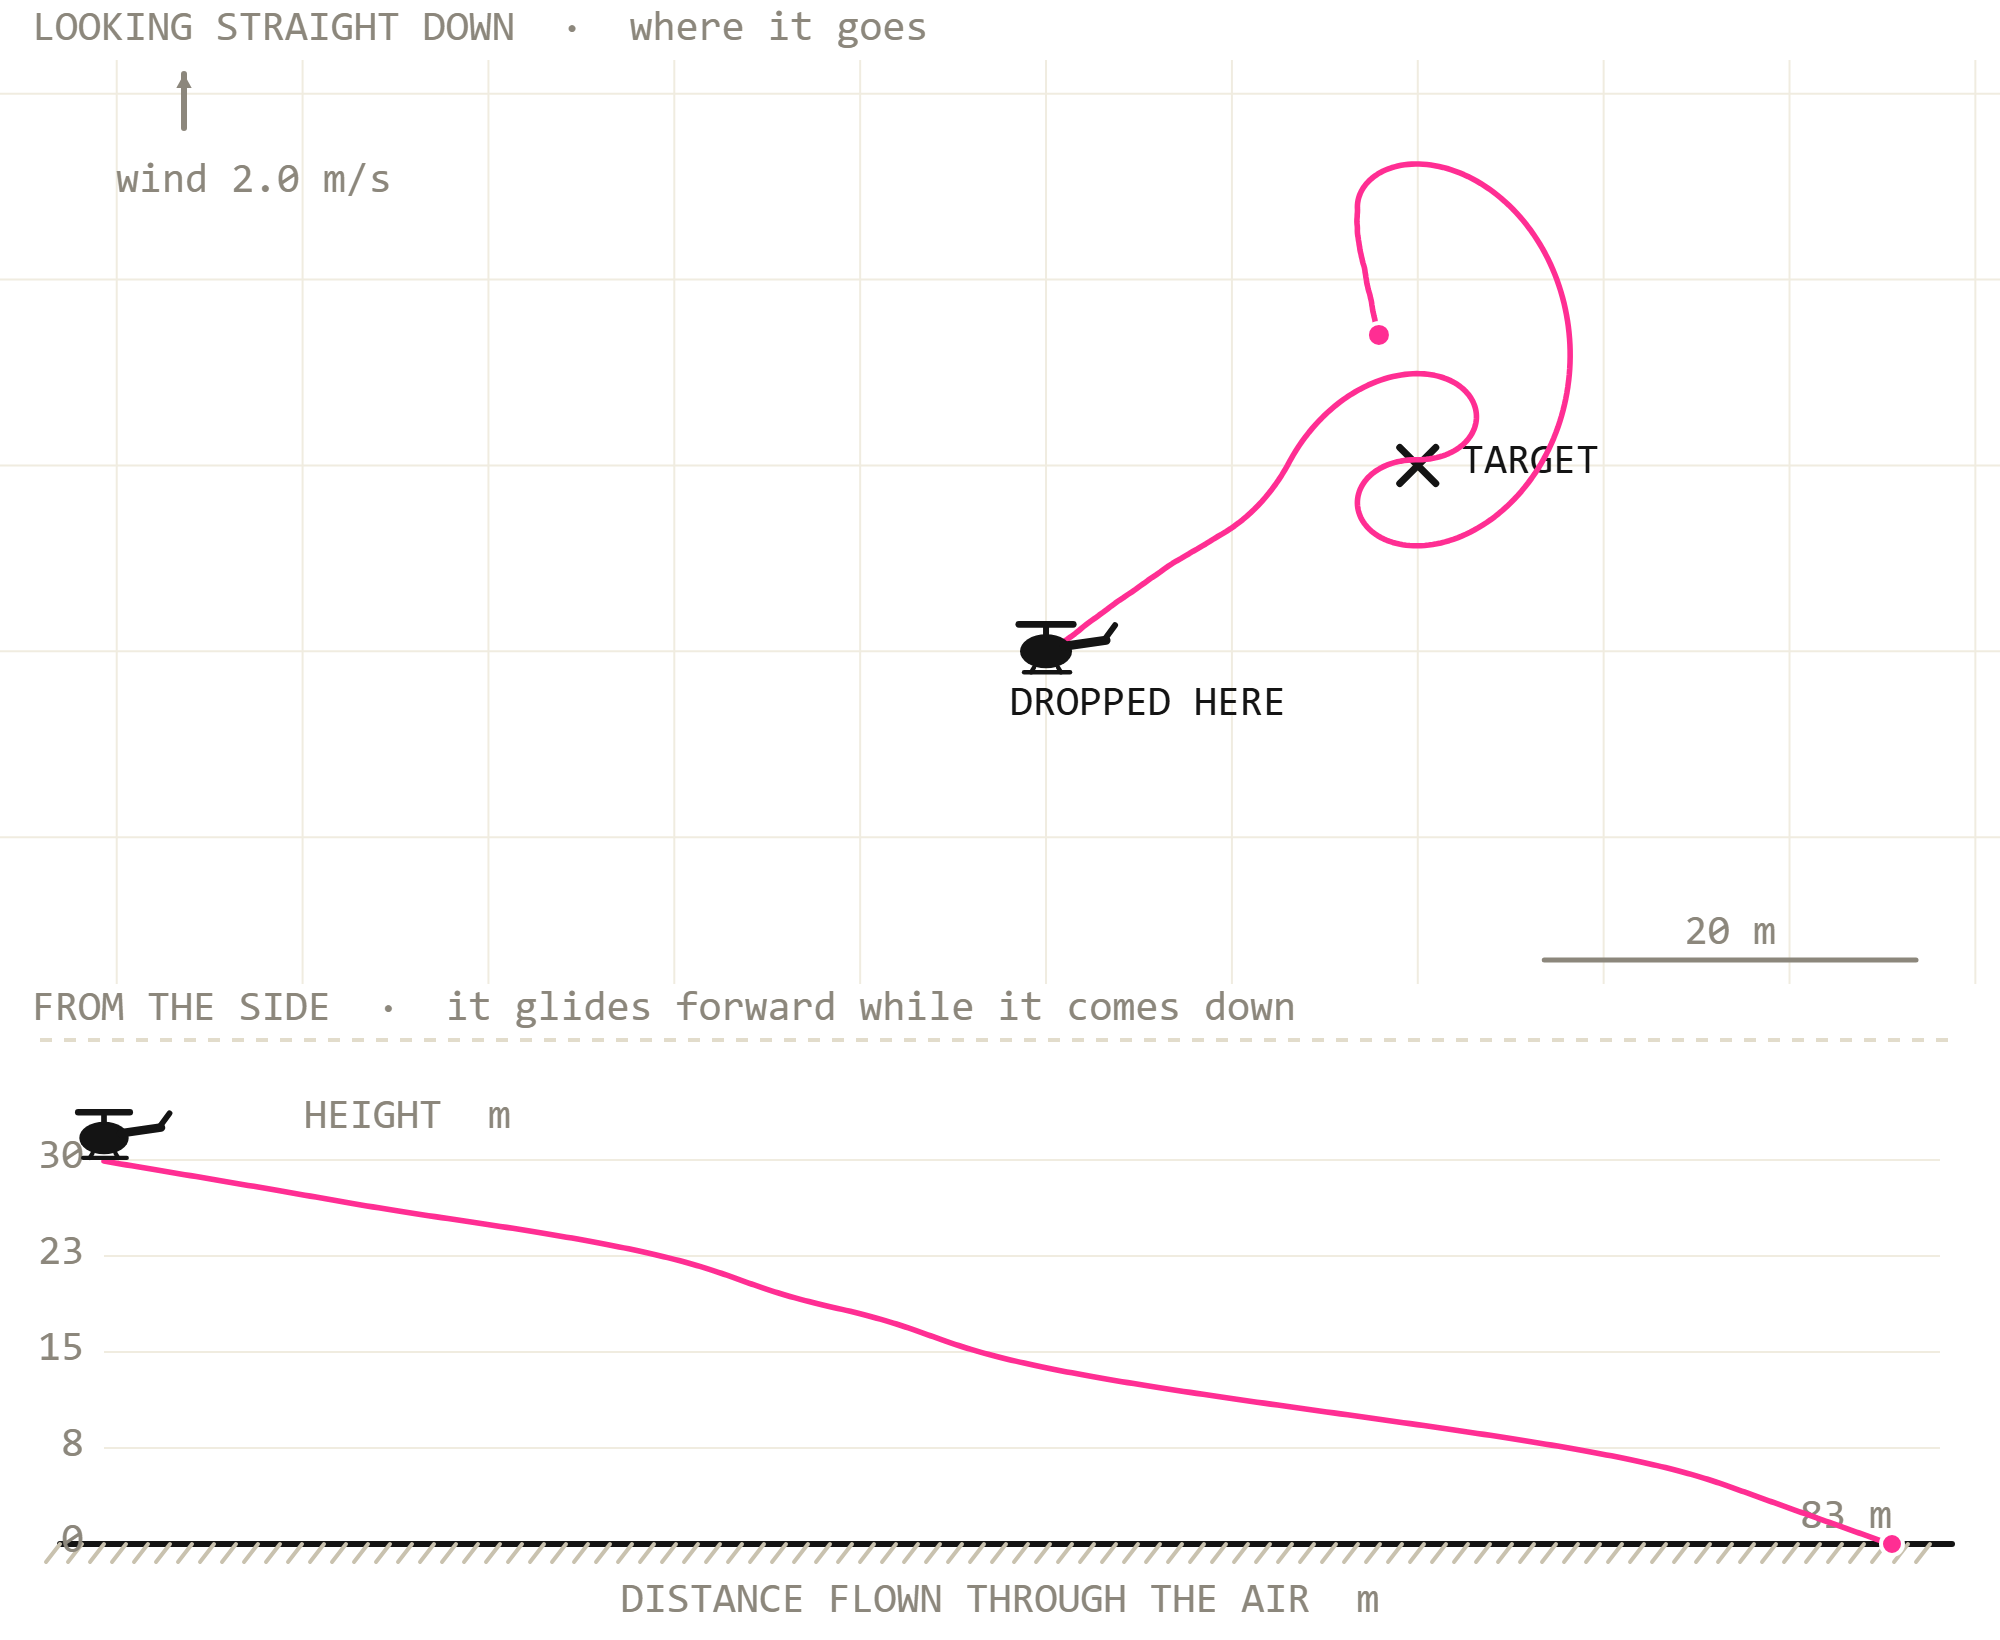
\includegraphics[width=\textwidth]{figures/drop_none.png}
  \caption{No wind estimate. Miss distance $7.33$~m.}
  \label{fig:drop-none}
\end{subfigure}\hfill
\begin{subfigure}[b]{0.49\textwidth}
  \centering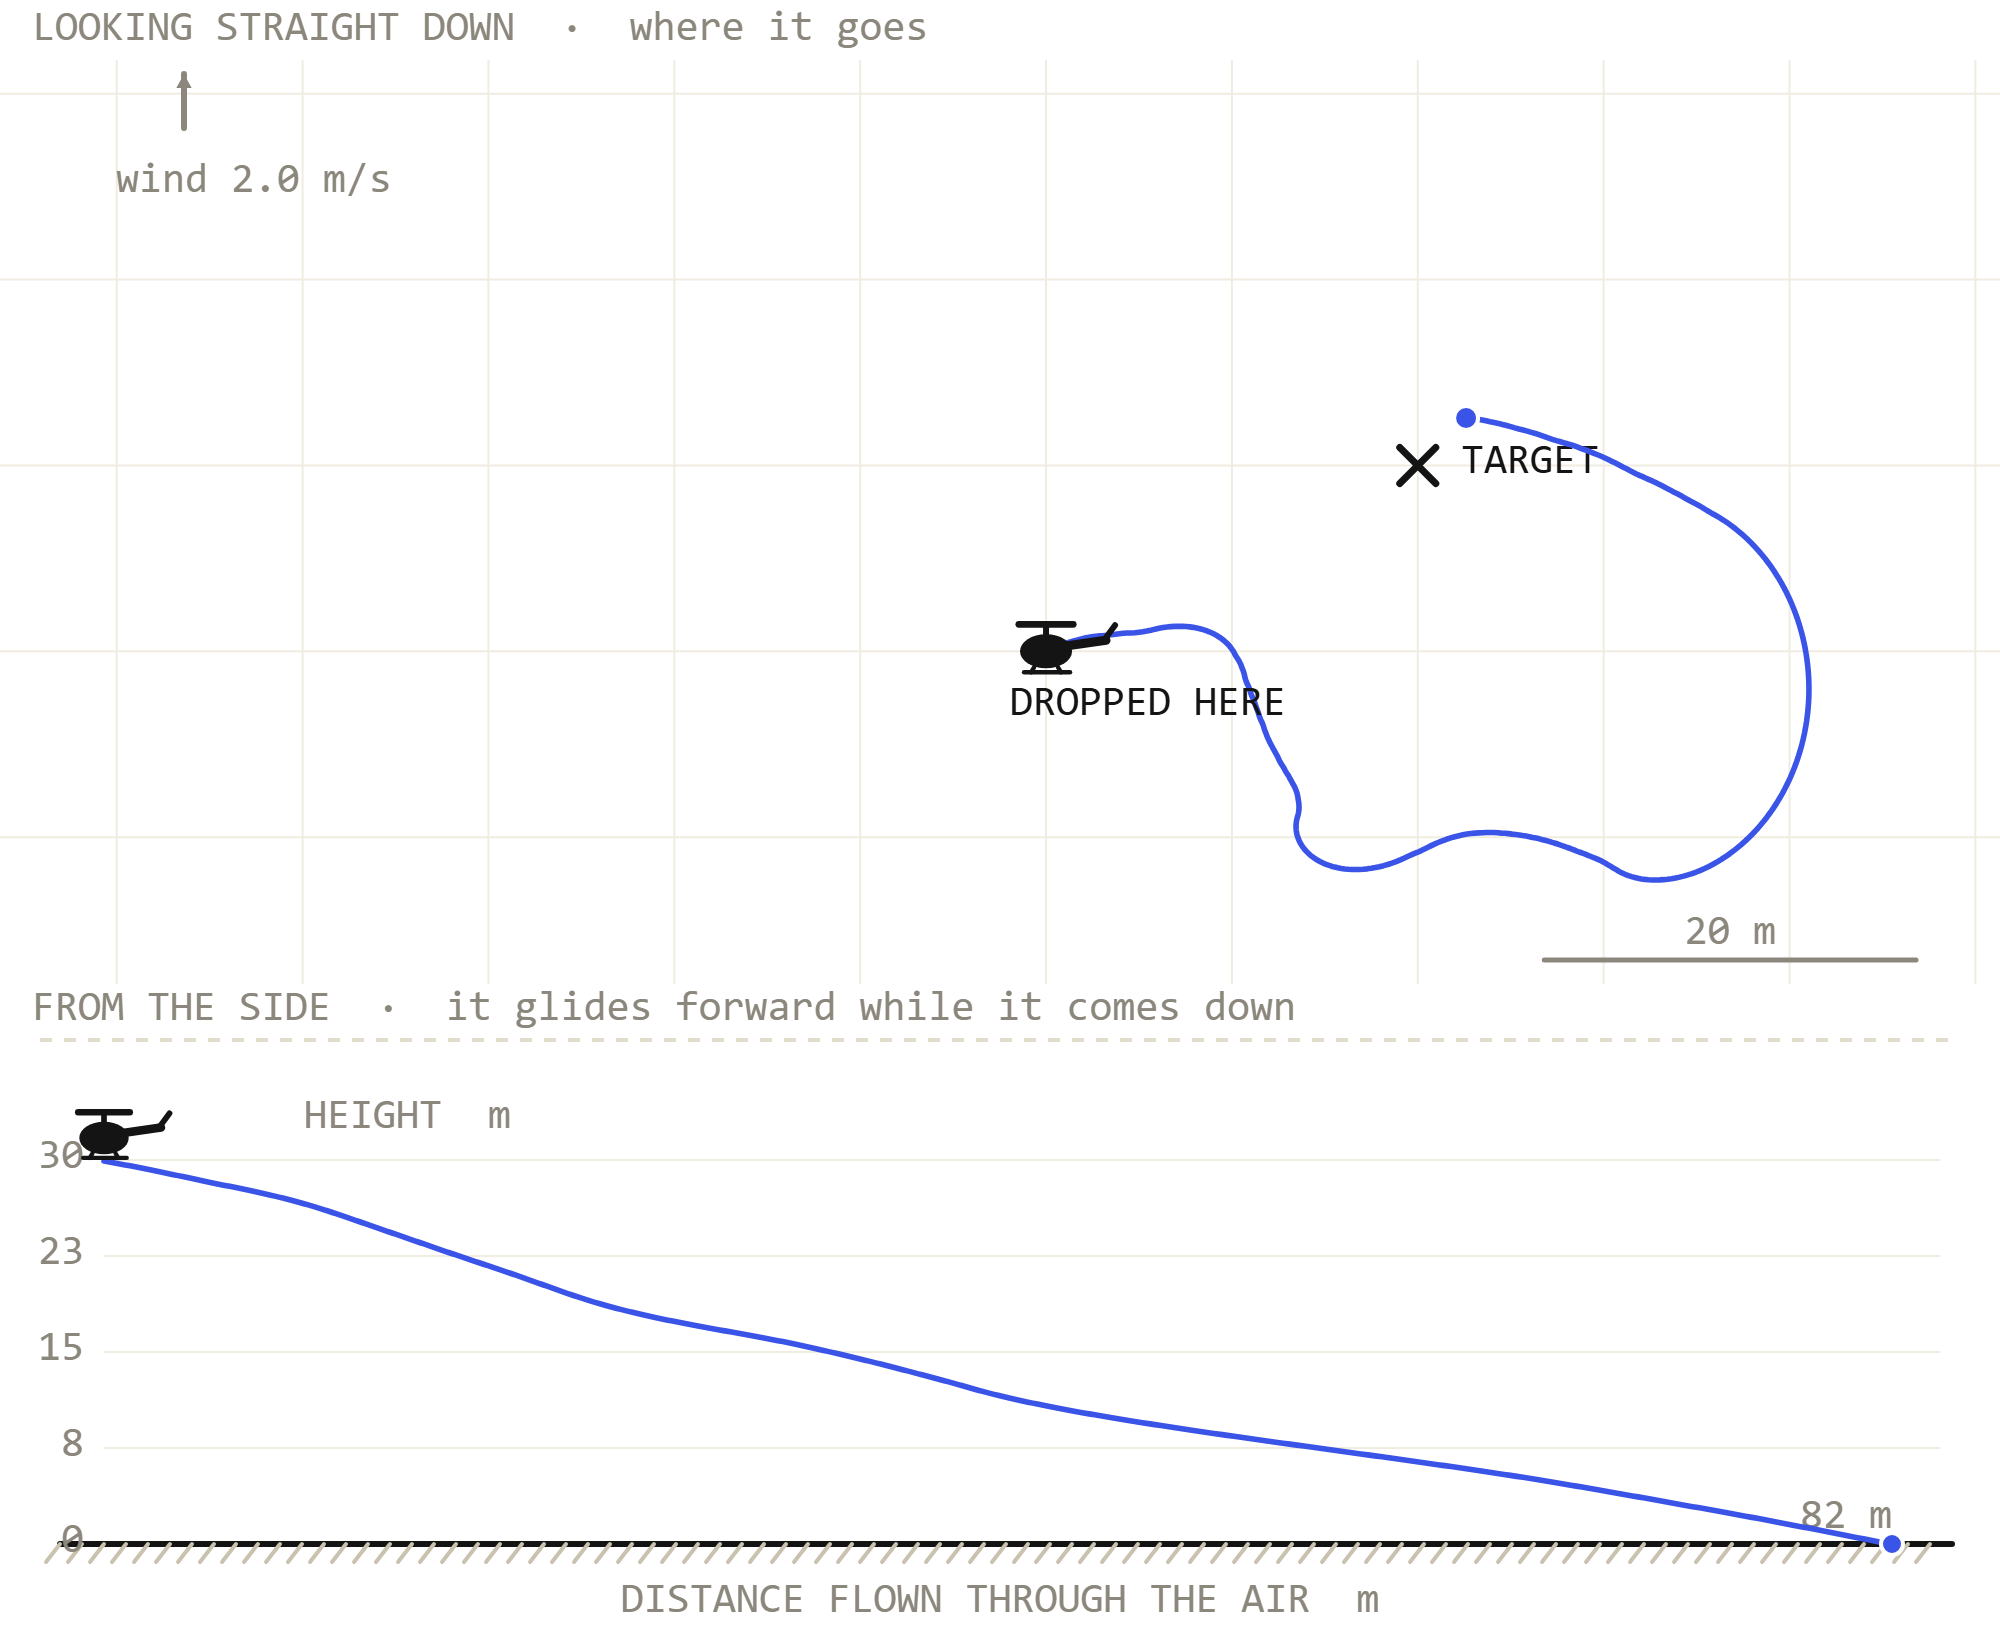
\includegraphics[width=\textwidth]{figures/drop_ekf.png}
  \caption{EKF estimate. Miss distance $3.64$~m.}
  \label{fig:drop-ekf}
\end{subfigure}
\caption{One descent, seen two ways, from the interactive model. The upper panel
of each pair is the flight from the side, projected onto the release--target
line, showing the canopy gliding forward as it descends at a constant rate; the
lower panel is the same flight from above, where the miss distance is exact in
both directions. The helicopter marks the release point, the flag and the cross
mark the target. The two figures share identical axes and identical conditions
--- wind $2.0$~m\,s$^{-1}$ from the south, release height $30$~m, wing loading
$1.2$~kg\,m$^{-2}$, magnetometer bias $+10^{\circ}$ --- differing only in whether
the guidance estimates the wind. These are single flights, shown to make the
trajectory concrete; the statistical comparison is in \cref{tab:results}. The
model can be flown interactively at
\url{https://1101-hub.github.io/guided-airdrop/}.}
\label{fig:drop}
\end{figure}

% ------------------------------------------------------------------ METHODS
\section{Methods}

\paragraph{Flight model.} As a point mass in steady glide with lift equal to
weight, the parafoil has airspeed
\begin{equation}\label{eq:v}
v \;=\; \sqrt{\frac{2g}{\rho C_L}}\;\sqrt{\frac{m}{S}},
\end{equation}
with $\rho$ air density, $C_L$ lift coefficient, $m$ payload mass, $S$ canopy
area; only the wing loading $m/S$ appears. When wind exceeds $v$ the vehicle is
advected downwind whatever the control input. Values used were $C_L = 0.80$,
$C_D = 0.27$ and $20^{\circ}$ bank.

\paragraph{Path planning.} Under a minimum turn radius the shortest route between
oriented configurations is a Dubins path: at most three turning or straight
segments in one of six orderings (Dubins, 1957). All six closed forms were
verified against step-wise integration (largest endpoint disagreement
$9.0\times10^{-12}$~m over $3{,}514$ solutions).


\paragraph{Path-length control.} Sink rate is constant, so time aloft and
distance flown are fixed at release: the path needs prescribed, not minimum,
length. A track at angle $\alpha$ to the bearing extends path length by
$1/\cos\alpha$, giving the law $\cos\alpha = d/s$ for remaining distance $d$ and
budget $s$; $\alpha$ alternates in sign. As altitude falls,
$d/s \to 1$ and $\alpha \to 0$, giving a straight final approach with no mode
change. Excess altitude is spent in a holding circle.


\paragraph{Wind estimation.} No wind sensor is carried. An EKF (Kalman, 1960)
maintains wind components $w_x$, $w_y$, airspeed $v_a$ and magnetometer bias $b$
from GNSS ground velocity, nonlinearity entering through $b$ in the heading
trigonometry. A headwind and an airspeed underestimate are indistinguishable on a
fixed heading, leaving the state unobservable; turning separates them, and
path-length control already turns.


\paragraph{Simulation.} Descent is integrated at $\Delta t = 0.05$~s, replanning
every step, and guidance sees only GNSS velocity with Gaussian noise of
$0.25$~m\,s$^{-1}$ and a magnetometer bias from $\pm12^{\circ}$, never the
simulated wind. Each trial draws wind $0$--$3.2$~m\,s$^{-1}$ with uniform heading
and release height $20$--$60$~m, flown three times under identical conditions:
\emph{no-estimate} (still air), \emph{EKF} (estimated onboard) and
\emph{true-wind} (supplied). \emph{Miss distance} is
horizontal separation between touchdown and target; intervals are bootstrap
percentiles from $20{,}000$ resamples.

% ------------------------------------------------------------------ RESULTS
\section{Results}

\begin{figure}[htbp]
\centering
\begin{subfigure}[b]{0.47\textwidth}
  \centering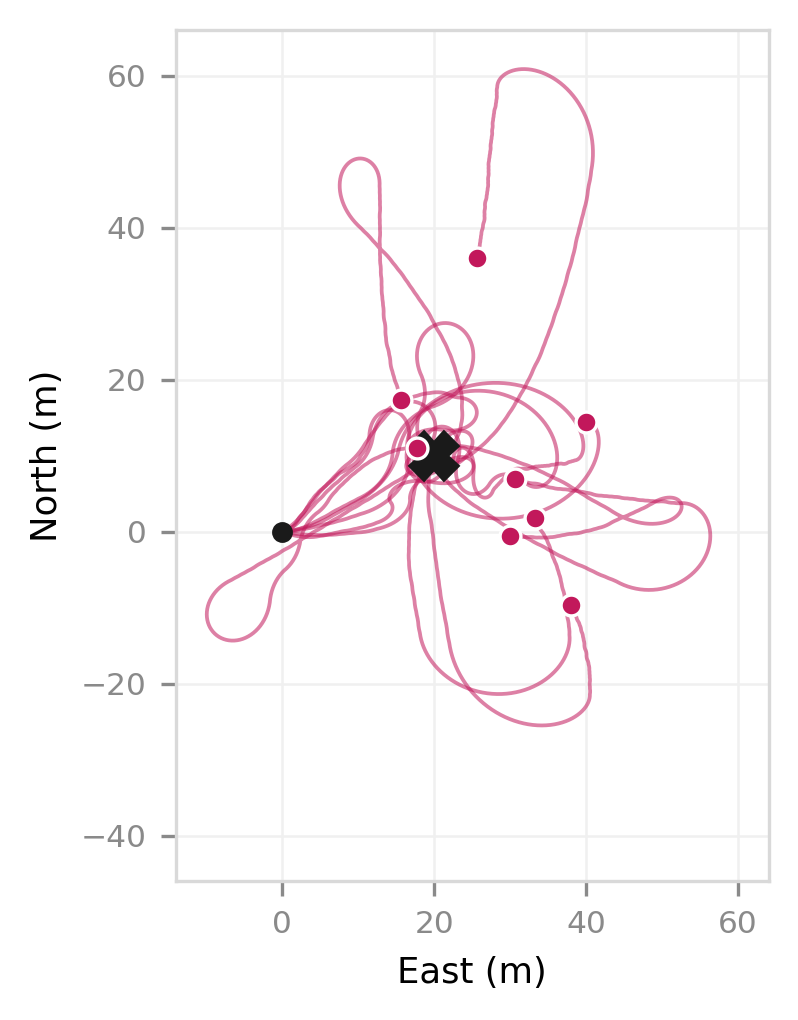
\includegraphics[width=\textwidth]{figures/fig1a_no_estimate.png}
  \caption{No-estimate configuration. Median miss distance $15.03$~m.}
  \label{fig:traj-none}
\end{subfigure}\hfill
\begin{subfigure}[b]{0.47\textwidth}
  \centering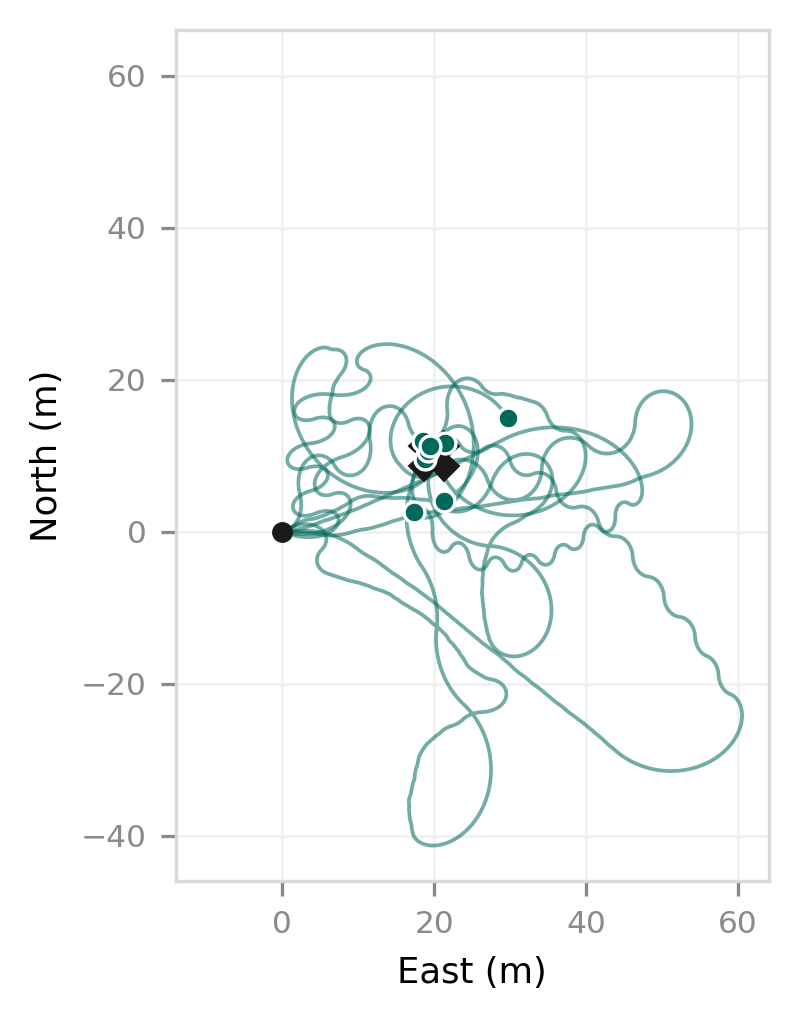
\includegraphics[width=\textwidth]{figures/fig1b_ekf_estimate.png}
  \caption{EKF configuration. Median miss distance $2.26$~m.}
  \label{fig:traj-ekf}
\end{subfigure}
\caption{Ground tracks of $N=8$ descents, plotted in a target-centred frame with
east and north in metres on identical axes in both panels. The same eight sets of
conditions are flown in each panel, with wind speed drawn from
$1.0$--$3.0$~m\,s$^{-1}$ and release height from $30$--$55$~m. The filled circle
at the origin marks release, the cross marks the target, and filled circles at
track ends mark touchdown. Touchdown points are dispersed in
\cref{fig:traj-none} and concentrated near the target in \cref{fig:traj-ekf}.}
\label{fig:traj}
\end{figure}

\Cref{fig:traj} shows eight descents per configuration; \cref{tab:results} covers
$N = 150$ randomised drops. Compared
trial by trial, the median reduction from adding the EKF is $4.26$~m ($95\%$ CI
$3.08$--$6.57$), and the EKF gives the smaller miss distance in $112$ of $150$
trials; wind velocity is recovered to a median error of $0.104$~m\,s$^{-1}$
($0.096$--$0.112$). The EKF and true-wind intervals overlap over most of their
range, so those configurations are not separated at this sample size.

\begin{table}[htbp]
\centering
\caption{Miss distance by guidance configuration over $N=150$ randomised drops.
Conditions are identical across rows and only the wind information available to
the guidance differs. Intervals on the median are $95\%$ bootstrap percentile
intervals; the uncertainty on the mean is the standard error.}
\label{tab:results}
\small
\begin{tabular}{lccc}
\toprule
Configuration & Median (m) & Mean (m) & $90$th percentile (m) \\
\midrule
No-estimate & $8.57$ ($6.49$--$12.46$) & $11.52 \pm 0.81$ & $24.27$ \\
EKF         & $3.89$ ($2.85$--$5.28$)  & $4.94 \pm 0.31$  & $10.75$ \\
True-wind   & $4.62$ ($3.37$--$5.44$)  & $4.84 \pm 0.32$  & $10.93$ \\
\bottomrule
\end{tabular}
\end{table}

Two scaling relations follow from \cref{eq:v}. Turn radius
$R = v^{2}/(g\tan\phi)$ at bank angle $\phi$, with $v \propto \sqrt{m/S}$,
gives $R \propto m/S$: across loadings $0.3$--$2.4$~kg\,m$^{-2}$ the ratio
$R/(m/S)$ is $4.7694$~m$^{3}$\,kg$^{-1}$, constant to $1.9\times10^{-14}\%$. Wind
penetration requires $v > W$, giving $(m/S)_{\min} \propto W^{2}$: for
$W = 2.0$--$4.0$~m\,s$^{-1}$ the ratio $(m/S)_{\min}/W^{2}$ is
$0.058722$~kg\,m$^{-2}$(m\,s$^{-1}$)$^{-2}$, constant to
$1.2\times10^{-14}\%$. Both sit at double-precision level: algebraic
identities, not fits. Composing them gives
\begin{equation}\label{eq:scaling}
R_{\min} \;\propto\; W^{2}.
\end{equation}
\Cref{fig:design} maps miss distance over this space.

\begin{figure}[htbp]
\centering
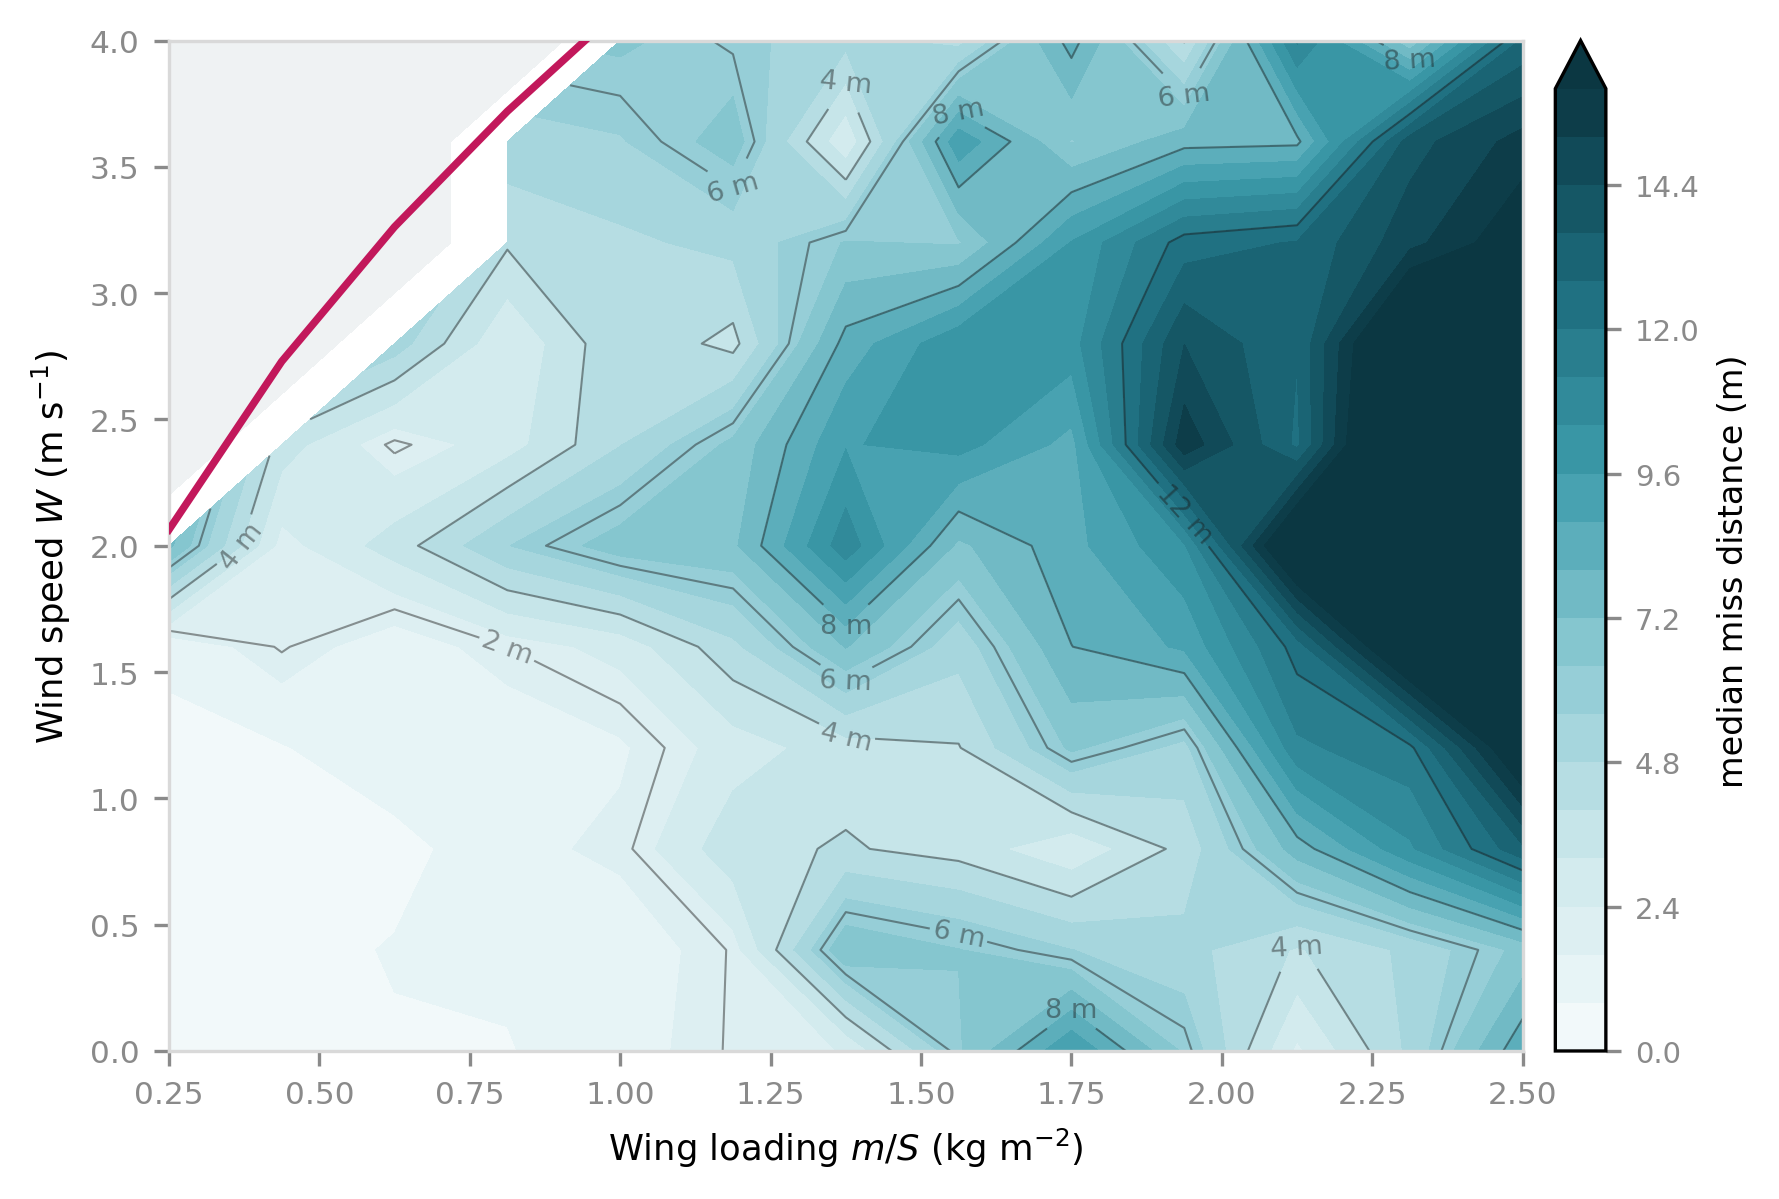
\includegraphics[width=0.82\textwidth]{figures/design_chart.png}
\caption{Median miss distance over wing loading $m/S$ and wind speed $W$, from
$24$ drops at each of $13\times11$ grid points in the EKF configuration at a
release height of $30$~m. Contours are labelled in metres. The line marks
$v = W$; in the shaded region below and left of it airspeed does not exceed wind
speed and no guided descent is possible. Miss distance is smallest at low wing
loading and low wind speed, and exceeds $12$~m at the highest loadings
irrespective of wind speed.}
\label{fig:design}
\end{figure}

% --------------------------------------------------------------- DISCUSSION
\section{Discussion}

The paired reduction establishes that onboard wind estimation improves accuracy
here. That the EKF is not separated from true-wind is consistent with its
correcting two error sources where true-wind corrects one: supplying wind leaves
the $\pm12^{\circ}$ magnetometer bias uncorrected, which the filter estimates
jointly. Separating them would need a larger sample.

\Cref{eq:scaling} follows from two competing requirements: penetrating wind of
speed $W$ demands a wing loading rising as $W^{2}$, while turn radius rises
linearly with loading and bounds the smallest correction achievable in the final
seconds. Specifying for wind never encountered therefore degrades accuracy in all
conditions, including calm. The appropriate choice is the lowest
loading satisfying $v > W$ with margin; set by ballast, it can be matched to the
forecast before release, unlike canopy area.

Three limitations bound these results: turbulence is absent, so the wind field is
uniform and steady and the accuracy reported is an upper bound; canopy
deformation is excluded, fixing $C_L$ and $C_D$; and actuator dynamics are
excluded, so turns begin instantaneously. Quantifying this optimism requires
flight measurement; the model specifies a test configuration ---
$1$~m$^{2}$ canopy, $0.5$--$0.8$~kg payload, $20$~m minimum release height ---
so it can be falsified rather than fitted.

% --------------------------------------------------------------- REFERENCES
\section*{References}
\small
ANI. (2026, July 25). \emph{IAF choppers deployed to airdrop essential relief
supplies in flood-affected areas: Assam CM Himanta Biswa Sarma}.

Daniel, K. (n.d.). \emph{ParaDrone: Autopilot for parachutes}.
\url{https://hackaday.io/project/176779-paradrone-autopilot-for-parachutes}

Dubins, L. E. (1957). On curves of minimal length with a constraint on average
curvature, and with prescribed initial and terminal positions and tangents.
\emph{American Journal of Mathematics, 79}(3), 497--516.

Kalman, R. E. (1960). A new approach to linear filtering and prediction problems.
\emph{Transactions of the ASME---Journal of Basic Engineering, 82}(D), 35--45.

Naval Postgraduate School. (n.d.). \emph{Snowflake}. Aerodynamic Decelerator
Systems Laboratory. \url{https://nps.edu/web/adsc/snowflake}

Onmanorama. (2026, July 25). \emph{Assam flood situation remains grim; toll rises
to 61, over 7 lakh affected}.

Tribune India. (2026, July 25). \emph{Govt yet to reach 80,000 flood victims,
says Assam CM; toll rises to 61}.

\end{document}
